\documentclass[class=llncs, crop=false]{standalone}
\usepackage{unicode-math}
\usepackage{newcomputermodern}
\usepackage{microtype}
\usepackage{newunicodechar}
\newunicodechar{⤳}{\ensuremath{⤳}}
\newunicodechar{↪}{\ensuremath{↪}}
\newunicodechar{≔}{\ensuremath{≔}}
\newunicodechar{⊢}{\ensuremath{⊢}}

% \usepackage{amsthm}
\usepackage{xcolor-material}
\usepackage{etoolbox}

%% ── Draft toggle ─────────────────────────────────────────────────
%% Comment out the next line for submission.
% \newcommand{\darkmode}{}

\ifdefined\darkmode
	\usepackage{showframe}
	\renewcommand\ShowFrameLinethickness{0.2pt}
	\renewcommand*\ShowFrameColor{\color{MaterialGrey600}}
	\usepackage{pagecolor}
	\pagecolor{MaterialGrey900}
	\color{MaterialGrey100}
\fi

\usepackage{tikz}
\usetikzlibrary{fit}
\usepackage{hyperref}
\ifdefined\darkmode
	\hypersetup{colorlinks=true,
		linkcolor=MaterialLightBlue300,
		citecolor=MaterialTeal300,
		urlcolor=MaterialLightBlue200}
\else
	\hypersetup{colorlinks=true,
		linkcolor=eoComment,
		citecolor=eoComment,
		urlcolor=eoComment}
\fi
\usepackage{ebproof}
\usepackage{array}

\usepackage{jbw-boxfigure}
\usepackage{jbw-fix-hyperref-autoref}

\usepackage{listings}
\usepackage[most]{tcolorbox}
\tcbuselibrary{listings}

%% ── Syntax colours ───────────────────────────────────────────────
\ifdefined\darkmode
	% Dark mode
	\definecolor{eoKeyword}{HTML}{f06292}%       commands   (pink)
	\definecolor{eoAttr}{HTML}{64b5f6}%          attributes (light blue)
	\definecolor{eoBuiltin}{HTML}{4dd0e1}%       builtins   (cyan)
	\definecolor{eoConst}{HTML}{b39ddb}%         types      (light purple)
	\definecolor{eoComment}{HTML}{9e9e9e}%       comments   (grey)
	\definecolor{eoString}{HTML}{ffb74d}%        strings    (light amber)
	\definecolor{eoPunct}{HTML}{bdbdbd}%         punctuation (light grey)
	\definecolor{eoFgMath}{HTML}{c8c0c8}%        foreground (softer)
\else
	% Light mode
	\definecolor{eoKeyword}{HTML}{e14775}%       commands   (pink)
	\definecolor{eoAttr}{HTML}{4a7fb5}%          attributes (muted blue)
	\definecolor{eoBuiltin}{HTML}{1c8ca8}%       builtins   (teal-cyan)
	\definecolor{eoConst}{HTML}{7058be}%         types      (purple)
	\definecolor{eoComment}{HTML}{3b5998}%       comments   (dark blue)
	\definecolor{eoString}{HTML}{cc7a0a}%        strings    (amber)
	\definecolor{eoPunct}{HTML}{918c8e}%         punctuation (grey)
	\definecolor{eoFgMath}{HTML}{3a3338}%        foreground (softer)
\fi

% Eunoia language definition for listings
\lstdefinelanguage{eunoia}{
	comment=[l]{;},
	string=[b]",
	morecomment=[s]{|}{|},% quoted symbols |...|
	alsoletter={-:@.},
	keywords={declare-const, declare-parameterized-const, declare-consts,
			declare-rule, declare-fun, declare-sort, declare-datatype,
			define, define-fun, define-const, define-sort,
			program, include, assume, assume-push, step, step-pop,
			let, match, as, par, forall, exists, lambda},
	keywords=[2]{:conclusion, :premises, :premise-list, :args,
			:requires, :assumption, :rule, :signature, :type,
			:right-assoc, :right-assoc-nil, :left-assoc, :left-assoc-nil,
			:chainable, :pairwise, :binder, :arg-list,
			:implicit, :opaque, :list, :sorry},
	% eo:: builtins handled via literate (see style below)
	keywords=[4]{Type, Proof},
	sensitive=true,
}

\lstdefinestyle{eo}{
language=eunoia,
basicstyle=\small\ttfamily\color{eoFgMath},
keywordstyle=\color{eoKeyword}\bfseries,
keywordstyle=[2]\color{eoAttr},
keywordstyle=[4]\color{eoConst},
commentstyle=\color{eoComment}\itshape,
stringstyle=\color{eoString},
showstringspaces=false,
columns=flexible,
keepspaces=true,
frame=none,
numbers=left,
numberstyle=\tiny\ttfamily\color{lineNoColor},
numbersep=6pt,
literate={(}{{\textcolor{eoPunct}{(}}}1
{)}{{\textcolor{eoPunct}{)}}}1
{[}{{\textcolor{eoPunct}{[}}}1
{]}{{\textcolor{eoPunct}{]}}}1
{eo::}{{\textcolor{eoBuiltin}{eo}\textcolor{eoPunct}{::}}}4
{$}{{\textcolor{eoConst}{\$}}}1,
	aboveskip=0.5\medskipamount,
	belowskip=0.5\medskipamount,
	}

	%% ── tcolorbox backgrounds ────────────────────────────────────────
	\ifdefined\darkmode
		\definecolor{eoBoxBg}{HTML}{2e3040}
		\definecolor{eoBoxFr}{HTML}{424454}
		\definecolor{lpBoxBg}{HTML}{2e3040}
		\definecolor{lpBoxFr}{HTML}{424454}
	\else
		\definecolor{eoBoxBg}{HTML}{fbfaf9}
		\definecolor{eoBoxFr}{HTML}{c5c1bf}
		\definecolor{lpBoxBg}{HTML}{fbfaf9}
		\definecolor{lpBoxFr}{HTML}{c5c1bf}
		\definecolor{lineNoColor}{HTML}{bfb9ba}
	\fi

	% tcolorbox style for Eunoia code blocks
	\newtcblisting{eolisting}{
		enhanced,
		listing only,
		listing options={style=eo, aboveskip=0pt, belowskip=0pt},
		colback=eoBoxBg,
		colframe=eoBoxFr,
		arc=0pt,
		boxrule=0.4pt,
		borderline west={1pt}{0pt}{eoBuiltin},
		left=14pt, right=2pt, top=2pt, bottom=2pt,
		before skip=\medskipamount,
		after skip=\medskipamount,
	}
	\newtcbinputlisting{\eofile}[1]{
		enhanced,
		listing only,
		listing file={#1},
		listing options={style=eo, aboveskip=0pt, belowskip=0pt},
		colback=eoBoxBg,
		colframe=eoBoxFr,
		arc=0pt,
		boxrule=0.4pt,
		borderline west={1pt}{0pt}{eoBuiltin},
		left=14pt, right=2pt, top=2pt, bottom=2pt,
		before skip=\medskipamount,
		after skip=\medskipamount,
		before upper=\listboxsetup,
	}

	% LambdaPi language definition and style
	\lstdefinelanguage{lambdapi}{
		comment=[l]{//},
		alsoletter={_},
		alsoother={@:$},
		keywords={symbol, rule, with, assert,
				require, open, type},
		keywords=[2]{constant, sequential, opaque, injective},
		keywords=[3]{TYPE},
		sensitive=true,
		mathescape=false,
		texcl=false,
	}

	\lstdefinestyle{lp}{
	language=lambdapi,
	basicstyle=\small\ttfamily\color{eoFgMath},
	keywordstyle=\color{eoKeyword}\bfseries,
	keywordstyle=[2]\color{eoAttr},
	keywordstyle=[3]\color{eoConst},
	commentstyle=\color{eoComment}\itshape,
	showstringspaces=false,
	columns=flexible,
	keepspaces=true,
	frame=none,
	numbers=left,
	numberstyle=\tiny\ttfamily\color{lineNoColor},
	numbersep=6pt,
	literate=
		{eo.Proof}{{\textcolor{eoBuiltin}{eo}\textcolor{eoPunct}{.}\textcolor{eoConst}{Proof}}}8
	{eo.app}{{\textcolor{eoBuiltin}{eo}\textcolor{eoPunct}{.}app}}6
	{eo.nil}{{\textcolor{eoBuiltin}{eo}\textcolor{eoPunct}{.}nil}}6
	{eo.}{{\textcolor{eoBuiltin}{eo}\textcolor{eoPunct}{.}}}3
	{eo::}{{\textcolor{eoBuiltin}{eo}\textcolor{eoPunct}{::}}}4
	{(}{{\textcolor{eoPunct}{(}}}1
	{)}{{\textcolor{eoPunct}{)}}}1
	{[}{{\textcolor{eoPunct}{[}}}1
	{]}{{\textcolor{eoPunct}{]}}}1
	{;}{{\textcolor{eoPunct}{;}}}1
	{:}{{\textcolor{eoPunct}{:}}}1
	{\{|}{{\textcolor{eoPunct}{\{|}}}2
	{|\}}{{\textcolor{eoPunct}{|\}}}}2
	{$}{{\textcolor{eoConst}{\$}}}1
{φ}{{$\varphi$}}1,
aboveskip=0.5\medskipamount,
belowskip=0.5\medskipamount,
}

% tcolorbox style for LambdaPi code blocks
\newtcblisting{lplisting}{
	enhanced,
	listing only,
	listing options={style=lp, aboveskip=0pt, belowskip=0pt},
	colback=lpBoxBg,
	colframe=lpBoxFr,
	arc=0pt,
	boxrule=0.4pt,
	borderline west={1pt}{0pt}{eoConst},
	left=14pt, right=2pt, top=2pt, bottom=2pt,
	before skip=\medskipamount,
	after skip=\medskipamount,
}
\newtcbinputlisting{\lpfile}[1]{
	enhanced,
	listing only,
	listing file={#1},
	listing options={style=lp, aboveskip=0pt, belowskip=0pt},
	colback=lpBoxBg,
	colframe=lpBoxFr,
	arc=0pt,
	boxrule=0.4pt,
	borderline west={1pt}{0pt}{eoConst},
	left=14pt, right=2pt, top=2pt, bottom=2pt,
	before skip=\medskipamount,
	after skip=\medskipamount,
	before upper=\listboxsetup,
}
% Thin separator line for use inside multi-part listing boxes
\newcommand{\listsep}{%
	\vspace{-\baselineskip}\vspace{7pt}%
	\noindent\kern-14pt\textcolor{eoBoxFr}{\rule{\dimexpr\linewidth+14pt+2pt}{0.3pt}}\par%
	\vspace{2pt}%
}
% Helper: zero out trivlist glue that listings inserts
\newcommand{\listboxsetup}{\topsep=0pt \partopsep=0pt \parsep=0pt \parskip=0pt}
% Multi-part listing boxes: use \listsep between \lstinputlisting calls
\newenvironment{eobox}{%
	\begin{tcolorbox}[
			enhanced, listing only,
			colback=eoBoxBg, colframe=eoBoxFr,
			arc=0pt, boxrule=0.4pt,
			borderline west={1pt}{0pt}{eoBuiltin},
			left=14pt, right=2pt, top=2pt, bottom=2pt,
			before skip=\medskipamount, after skip=\medskipamount,
		]\listboxsetup
		}{\end{tcolorbox}}
\newenvironment{lpbox}{%
	\begin{tcolorbox}[
			enhanced, listing only,
			colback=lpBoxBg, colframe=lpBoxFr,
			arc=0pt, boxrule=0.4pt,
			borderline west={1pt}{0pt}{eoConst},
			left=14pt, right=2pt, top=2pt, bottom=2pt,
			before skip=\medskipamount, after skip=\medskipamount,
		]\listboxsetup
		}{\end{tcolorbox}}
\lstset{defaultdialect=[]{eunoia}}

% Redefine example and definition to use italic headings
\let\example\relax
\let\endexample\relax
\spnewtheorem{example}{Example}{\itshape}{\rmfamily}
\def\exampleautorefname{example}
\let\definition\relax
\let\enddefinition\relax
\spnewtheorem{definition}{Definition}{\itshape}{\rmfamily}

\usepackage[backend=biber]{biblatex}
\addbibresource{inria.bib}

% small cases environment (brace + contents scaled to \small)
\newenvironment{scases}{%
	\left\{\,\small\begin{array}{@{}l@{\quad}l@{}}%
		}{%
	\end{array}\right.%
}

% font faces
\newcommand{\msf}{\mathsf}
\newcommand{\mbf}{\mathbf}
\newcommand{\mscr}{\mathscr}
\newcommand{\mtt}[1]{{\color{eoConst}{\texttt{#1}}}}% types/constants: Type, Bool, true, false, Proof
\newcommand{\kw}[1]{{\color{eoKeyword}{\texttt{\textbf{#1}}}}}% commands: declare-const, define, program, ...
\newcommand{\ev}[1]{{\color{eoFgMath}{\texttt{#1}}}}
\newcommand{\equo}{{\color{eoString}{\texttt{"}}}}% string quote
\newcommand{\estr}[1]{\equo{#1}\equo}% string literals

\newcommand{\cpc}{\msf{CPC}}
\newcommand{\tsm}[1]{{\small\text{#1}}}

\newcommand{\ptn}[1]{{\color{MaterialPurple500}{\texttt{#1}}}}
\newcommand{\mcomment}[1]{{\color{MaterialIndigo500}{\text{#1}}}}
\newcommand{\wrapp}[4]{{\color{#1}{#2}}{#4}{\color{#1}{#3}}}
\newcommand{\prn}[1]{\wrapp{MaterialGrey600}{\lparen}{\rparen}{#1}}

\newcommand{\cvc}[1]{\textsc{cvc{#1}}}
\newcommand{\verit}{\textsc{veriT}}
\newcommand{\eunoia}{\textsc{Eunoia}}

% ----- abstract syntax ----------
% plurality, binding
\newcommand{\plur}[2]{{#1}_{1}\ldots{#1}_{#2}}
\newcommand{\plurcomma}[2]{{#1}_{1}, \ldots, {#1}_{#2}}
\newcommand{\maybe}[1]{\wrapp{MaterialGrey600}{\langle}{\rangle_?}{#1}}
\newcommand{\many}[1]{\wrapp{MaterialGrey600}{\langle}{\rangle_+}{#1}}
\newcommand{\any}[1]{\wrapp{MaterialGrey600}{\langle}{\rangle_∗}{#1}}
\newcommand{\some}[1]{\wrapp{MaterialGrey600}{\langle}{\rangle}{#1}}
\newcommand{\binddot}[3]{{#1\,#2.\,#3}}

% binders
\newcommand{\lam}{\binddot{λ}}
\newcommand{\pii}{\binddot{Π}}
\newcommand{\alam}[1]{\binddot{\msf{λ}^{#1}}}
\newcommand{\apii}[1]{\binddot{\msf{Π}^{#1}}}
\newcommand{\lett}[2]{\msf{let}\ \prn{#1}\,\msf{in}\ #2}

% applications
\newcommand{\appSym}{\cdot}
\newcommand{\app}[2]{{#1}\appSym{#2}}
\newcommand{\apptwo}[3]{#1\,#2\,#3}
\newcommand{\appthree}[4]{#1\,#2\,#3\,#4}
\newcommand{\appfour}[5]{#1\,#2\,#3\,#4\,#5}
\newcommand{\appldots}[3]{\prn{\prn{\app{#1}{#2}}\,\ldots\,⋅\,{#3}}}

% universes
\newcommand{\PROP}{\mtt{PROP}}
\newcommand{\TYPE}{\mtt{TYPE}}
\newcommand{\KIND}{\mtt{KIND}}



% -------------- Eunoia ------------------------------------
% eunoia symbols
\newcommand{\epar}[1]{\wrapp{eoPunct}{\texttt{(}}{\texttt{)}}{#1}}
\newcommand{\eapp}[2]{\epar{#1\ #2}}
\newcommand{\earr}[1]{\epar{\ev{->}\ #1}}
\newcommand{\eprf}[1]{\epar{\mtt{Proof}\ #1}}
\newcommand{\ecase}[2]{\epar{#1\ #2}}
\newcommand{\eo}[1]{{\color{eoBuiltin}{\texttt{eo}}}{\color{eoPunct}{∷}}{\ev{#1}}}% builtins
\newcommand{\eotype}{\mtt{Type}}
\newcommand{\eoreqs}[3]{\eapp{\eo{requires}}{#1\ #2\ #3}}
\newcommand{\eoquote}[1]{\eapp{\eo{quote}}{#1}}

\newcommand{\attr}[1]{{\color{eoAttr}{\texttt{:#1}}}}% attributes
\newcommand{\premises}[1]{\attr{premises}\,\epar{#1}}
\newcommand{\premiselist}[2]{\attr{premise-list}\ #1\ #2}
\newcommand{\requires}[1]{\attr{requires}\ \epar{#1}}
\newcommand{\conclusion}[1]{
	\attr{conclusion}\ #1
}


\newcommand{\sym}[1]{\msf{s}_{\msf{#1}}}
% \newcommand{\eoapp}[2]{\prn{#1\ #2}}
% \newcommand{\earr}[1]{\mtt{#1}}
\newcommand{\ctyp}{\mbf{ctyp}}
\newcommand{\att}{\mbf{att}}

\newcommand{\prf}{\mbf{prf}}
\newcommand{\step}{\mbf{step}}

\newcommand{\eor}{\texttt{or}}
\newcommand{\econcat}[3]{\eapp{\eo{list\_concat}}{#1\ #2\ #3}}
\newcommand{\econs}[3]{\eapp{#1}{#2\ #3}}
\newcommand{\false}{\texttt{false}}

\newcommand{\rcn}[1]{\attr{right-assoc-nil}\ {#1}}
\newcommand{\rc}{\attr{right-assoc}}

\newcommand{\lcn}[1]{\attr{left-assoc-nil}\ {#1}}
\newcommand{\lc}{\attr{left-assoc}}

\newcommand{\ch}[1]{\attr{chainable}\ {#1}}
\newcommand{\pw}[1]{\attr{pairwise}\ {#1}}
\newcommand{\bd}[1]{\attr{binder}\ {#1}}
\newcommand{\al}[1]{\attr{arg-list}\ {#1}}
\newcommand{\eovar}[2]{\eapp{\eo{var}}{#1\ #2}}

% --- builtin operators (sec:eo-builtin) ---
\newcommand{\eoBuiltinFig}{
	\begin{array}[t]{r@{\ }l@{\ }l@{\quad}l}
		β & {⦂}
		  & \eo{ite}\ ∣\ \eo{eq}\ ∣\ \eo{requires}\ ∣\ \eo{typeof}\ ∣\ \eo{var}\ ∣\ \ldots
		  & \mcomment{(core)}
		\\
		  & {∣}
		  & \eo{and}\ ∣\ \eo{or}\ ∣\ \eo{not}\ ∣\ \eo{xor}
		  & \mcomment{(boolean)}
		\\
		  & {∣}
		  & \eo{add}\ ∣\ \eo{mul}\ ∣\ \eo{neg}\ ∣\ \eo{zdiv}\ ∣\ \ldots
		  & \mcomment{(arithmetic)}
		\\
		  & {∣}
		  & \eo{nil}\ ∣\ \eo{cons}\ ∣\ \eo{list\_concat}\ ∣\ \eo{list\_len}\ ∣\ \ldots
		  & \mcomment{(list)}
	\end{array}
}


\newcommand{\cons}{{\text{cons}}}
\newcommand{\nil}{{\text{nil}}}
\newcommand{\foldl}{\mbf{foldl}}
\newcommand{\foldr}{\mbf{foldr}}
\newcommand{\elab}[1]{\mbf{elab}_{\prn{#1}}}
\newcommand{\glue}[1]{\mbf{glue}_{\prn{#1}}}
\newcommand{\bool}{\texttt{Bool}}
% ---- eo commands ------
\newcommand{\dc}[2]{\epar{\kw{declare-const}\ {#1}\ {#2}}}
\newcommand{\dca}[3]{\epar{\kw{declare-const}\ {#1}\ {#2}\ {#3}}}

% --- figures for `eoas.tex` ------------------------------
% s & {⦂}\ \sym 0 ∣ \sym 1 ∣ \ldots
% 		& \mcomment{(symbols)}         &
%
\newcommand{\eoTermSyntax}{
	\begin{array}[t]{r@{\ }l@{\quad}l@{\qquad}r@{\ }l@{\quad}l}
		%!----------------------------------------!%
		t & {⦂}\ s \mid ℓ \mid \eapp{s}{\vec t} \mid \eapp{s}{\epar{\vec{ρ}}\ t} & \mcomment{(terms)}      &
		ρ & {⦂}\ \epar{s\ t\ \maybe{ν}}                                          & \mcomment{(parameters)}   \\[1mm]
		ℓ & {⦂}\ \msf{int}(n) ∣ \msf{str}(s)                                     & \mcomment{(literals)}   &
		c & {⦂}\ \epar{t\ t'}                                                    & \mcomment{(cases)}        \\[1mm]
	\end{array}
}

\newcommand{\eoAttrSyntax}{
	\begin{array}[t]{r@{\ }c@{\ }l@{\quad}l}
		ν & {⦂} & \attr{implicit} \mid \attr{list}               & \mcomment{(prm. attributes)}   \\
		α & {⦂} & \attr{right-assoc} ∣ \attr{right-assoc-nil}\ t & \mcomment{(const. attributes)} \\
		  & {∣} & \attr{left-assoc} ∣ \attr{left-assoc-nil}\ t                                    \\
		  & {∣} & \attr{chainable}\ s ∣ \attr{pairwise}\ s                                        \\
		  & {∣} & \attr{binder}\ s ∣ \attr{arg-list}\ s
	\end{array}
}

\newcommand{\eoCommandSyntax}{
	\begin{array}[t]{r@{\ }l@{\quad}l}
		δ & \begin{array}[t]{c@{\ }l}
			    {⦂} & \epar{\kw{declare-const}\ s\ t\ \maybe{α}}                               \\
			    {∣} & \epar{\kw{declare-parameterized-const}\ s\ \epar{\vec{ρ}}\ t\ \maybe{α}} \\
			    {∣} & \epar{\kw{declare-consts}\ ℓ\ t}                                         \\
			    {∣} & \epar{\kw{define}\ {s} \ \epar{\vec ρ} \ t\ \ \maybe{\attr{type}\,t'}}   \\
			    {∣} & \epar{\kw{program}\ {s} \ \epar{\vec ρ}\
			    \attr{signature}\,\epar{\vec{t}}\,t'\
			    \epar{\vec{c}}
			    }                                                                              \\
			    {∣} & {\color{eoPunct}{\texttt{(}}}
			    \kw{declare-rule}\ s\ \epar{\vec ρ}\
			    \\ & \quad \maybe{\attr{assumption}\ t_{\text{assm}}}\
			    \\ & \quad \maybe{
			    \attr{premises}\ \epar{\vec{t}_{\text{prem}}}
			    \mid
			    \attr{premise-list}\ t_{\text{prem}}\ t_{\text{op}}
			    }\
			    \\ & \quad \maybe{\attr{args}\ \epar{\vec{t}_{\text{args}}}}\
			    \\ & \quad \maybe{\attr{requires}\ \epar{\vec{c}}}\
			    \\ & \quad \attr{conclusion}\ {t_{\text{conc}}}
			    {\color{eoPunct}{\texttt{)}}}                                                  \\
			    {∣} & \epar{\kw{include}\ μ}
		    \end{array}
		  & \mcomment{(std. commands)}
	\end{array}
}

\newcommand{\eoPrfCommandSyntax}{
	\begin{array}[t]{r@{\ }l@{\quad}l}
		π & \begin{array}[t]{c@{\ }l}
			    {⦂} & \epar{\kw{assume}\ s\ φ}      \\
			    {∣} & \epar{\kw{assume-push}\ s\ φ} \\
			    {∣} & \epar{\kw{step}\ s\ φ\
			    \attr{rule}\ s'\
			    \maybe{\attr{premises}\ {\vec ψ}}\
			    \maybe{\attr{args}\ {\vec t}}}      \\
			    {∣} & \epar{\kw{step-pop}\ s\ φ\
			    \attr{rule}\ s'\
			    \maybe{\attr{premises}\ {\vec ψ}}\
			    \maybe{\attr{args}\ {\vec t}}}      \\
		    \end{array}
		  & \mcomment{(prf. commands)}
	\end{array}
}

%
%
% --- macros for `lp.tex` ------------------------------
\newcommand{\esc}[1]{\wrapp{MaterialGrey600}{⦃}{⦄}{#1}}
\newcommand{\var}[1]{\msf{v}_{#1}}
\newcommand{\lbl}[2]{\rname{#1}\quad{#2}}
\newcommand{\lpTermSyntax}{
	\begin{array}[t]{r@{\ }l@{\quad}r}
		% ------------------------------------- %
		μ & {⦂}\ \TYPE ∣ \KIND
		  & \mcomment{(universes)}                                                             \\[1mm]
		% ------------------------------------- %
		t & {⦂}\ x ∣ κ ∣ μ ∣ \prn{\app{t}{t'}} ∣ \prn{\lam{x : t}{t'}} ∣ \prn{\pii{x : t}{t'}}
		  & \mcomment{(terms)}
		% ------------------------------------- %
	\end{array}
}

\newcommand{\lpCtxSyntax}{
	\begin{array}[t]{r@{\ }l@{\quad}r}
		% ------------------------------------- %
		γ & {⦂}\ \prn{x : t} \mid \prn{t ↪ t'} \
		  & \mcomment{(context elements)}        \\
		% ------------------------------------- %
		Γ & {⦂}\ \any{γ}
		  & \mcomment{(contexts)}
		% ------------------------------------- %
	\end{array}
}

\newcommand{\judge}[3]{{#1} ⊢_{Σ} {#2} : {#3}}
\newcommand{\wf}[1]{\msf{wf}\,{#1}}
% typing rules
\newcommand{\typeRule}{
	\begin{prooftree}
		\hypo{\wf Γ}
		\infer1{ \judge Γ \TYPE \KIND }
	\end{prooftree}
}

\newcommand{\varRule}{
	\begin{prooftree}
		\hypo{ \wf Γ}
		\infer1[$\prn{x : t}∈ Γ$]{ \judge Γ x t }
	\end{prooftree}
}

\newcommand{\constRule}{
	\begin{prooftree}
		\hypo{\wf Γ}
		\hypo{\judge {} t μ}
		\infer2[$\prn{κ : t}∈ Σ$]{ \judge Γ κ t }
	\end{prooftree}
}

\newcommand{\prodRule}{
	\begin{prooftree}
		\hypo{\judge Γ t {\TYPE}}
		\hypo{\judge{Γ, \prn{x : t}}{t'}{μ'}}
		\infer2{\judge Γ {\prn{\pii {x : t} {t'}}} {μ'} }
	\end{prooftree}
}

\newcommand{\absRule}{
	\begin{prooftree}
		\hypo{\judge{Γ, \prn{x : t}} e {t'}}
		\hypo{\judge Γ {\prn{\pii {x : t} {t'}}} μ}
		\infer2{\judge Γ {\prn{\lam {x : t} {e}}} {\prn{\pii {x : t} {t'}}} }
	\end{prooftree}
}

\newcommand{\appRule}{
	\begin{prooftree}
		\hypo{\judge Γ e {\prn{\pii{x : t}{t'}}}}
		\hypo{\judge Γ {e'} t}
		\infer2{\judge Γ {\prn{\app{e}{e'}}} {t'[x ↦ {e'}]}}
	\end{prooftree}
}

\newcommand{\convRule}{
	\begin{prooftree}
		\hypo{\judge Γ e t}
		\hypo{\judge Γ {t'} {μ}}
		\infer2[$\prn{t ≡_{βΣ} t'}$]{\judge Γ {e} {t'}}
	\end{prooftree}
}

\newcommand{\wfRuleEmp}{
	\begin{prooftree}
		\infer0{ \wf{\msf{∅}} }
	\end{prooftree}
}

\newcommand{\wfRuleVar}{
	\begin{prooftree}
		\hypo{ \judge Γ t μ }
		\infer1[$x ∉ \mbf{dom}(Γ)$]{ \wf{(Γ, \prn{x : t})}}
	\end{prooftree}
}

\newcommand{\rname}[1]{\mcomment{($\textsc{#1}$)}}

\newcommand{\lpTypingRules}{
	\begin{array}[t]{c}
		\lbl{wf0}{\wfRuleEmp} \qquad \lbl{wf+}{\wfRuleVar}
		\\[6mm]
		\lbl{var}{\varRule}    \qquad  \lbl{con}{\constRule}
		\\[6mm]
		\lbl{univ}{\typeRule}  \qquad \lbl{prod}{\prodRule}
		\\[6mm]
		\lbl{fun}{\absRule} \\[6mm]
		\lbl{app}{\appRule} \\[6mm]
		\lbl{conv}{\convRule}
	\end{array}
}



% --- concrete syntax for lambdapi
\newcommand{\lambdapi}{\textsc{LambdaPi}}
\newcommand{\llam}{\binddot{\msf{λ}}}
\newcommand{\ppii}{\binddot{\msf{Π}}}

% \newcommand{\symbol}{\mtt{symbol}}

\newcommand{\prm}[1]{\mbf{#1}}
\newcommand{\xsym}[1]{\mtt{@}{#1}}
\newcommand{\meta}[1]{\ptn{?{#1}}}

\newcommand{\ptrn}[1]{\ptn{\$#1}}
\newcommand{\pv}{\mbf{pvars}}

\newcommand{\imp}[1]{[#1]}
\newcommand{\xpl}[1]{\left(#1\right)}

\newcommand{\lpTermsConcrete}{
	\begin{array}[t]{r@{\ }l@{\quad}r}
		t & {⦂}\ s ∣ \imp{t} ∣ \prn{\app{t}{t'}}
		∣ \prn{\llam{ρ}{t}} ∣ \prn{\ppii{ρ}{t}}
		  & \mcomment{(terms)}
	\end{array}
}

\newcommand{\lpPatternSyntax}{
	\begin{array}[t]{r@{\ }c@{\ }l@{\quad}r@{\qquad}r@{\ }c@{\ }l@{\quad}r}
		m & {⦂}
		  & \mtt{constant} ∣ \mtt{sequential}
		  & \mcomment{(modifiers)}
		  &
		θ & {⦂}
		  & \ptrn{x} ∣ s\,\any{θ}
		  & \mcomment{(patterns)}
		\\[1mm]
		ρ & {⦂}
		  & \xpl{s : t} ∣ \imp{s : t}
		  & \mcomment{(parameters)}
		  &
		% ------------------------------------- %
		r & {⦂}
		  & \prn{{s\,\any{θ}} ↪ {θ'}}
		  & \mcomment{(rewrite rules)}
		% ------------------------------------- %
	\end{array}
}

\newcommand{\lpConcreteSyntax}{
	\begin{array}[t]{r@{\ }c@{\ }l@{\quad}r}
		c & {⦂}
		  & \maybe{m}\, \mtt{symbol}\ s \ \any{ρ} \,{: t} \ \maybe{≔ t'};
		  & \mcomment{(commands)}
		\\
		  & {∣}
		  & \mtt{rule}\ r\ \any{\mtt{with}\ r'};
		\\
		  & {∣}
		  & \mtt{require}\,\mtt{open}\,\many{μ};
	\end{array}}

% \newcommand{\symb}[1]{\mtt{symbol}\ {#1};}

% \newcommand{\symb}[1]{\mtt{rule}\ {#1};}

\newcommand{\Set}{\msf{Set}}
\newcommand{\El}[1]{\msf{τ}\,{#1}}

% ------- translation stuff -----------
\newcommand{\Term}{\msf{Term}}

%
\newcommand{\EO}{\msf{EO}}
\newcommand{\LP}{\msf{LP}}
\newcommand{\trans}[1]{\left⟦{#1}\right⟧}
\newcommand{\tm}[1]{\trans{#1}_\msf{tm}}
\newcommand{\ty}[1]{\trans{#1}_\msf{ty}}
\newcommand{\cmd}[1]{\trans{#1}_\msf{cmd}}
\newcommand{\ctx}[1]{\trans{#1}_\msf{ctx}}


\begin{document}
\section{Introduction}\label{sec:intro}
%
The area of automated reasoning known as
\emph{satisfiability modulo theories} (SMT)
focuses on the development of tools for
checking the satisfiability of first-order
formulas over combinations of mathematical
theories~\cite{Barrett2021}.
%
Such tools (known as SMT \emph{solvers}) are
increasingly used as back-ends for various tasks:
hardware~\cite{DBLP:conf/fmcad/MattareiMBDHH18} and
software verification~\cite{barnett06boogie,riant23debugging,kosmatov16frama-c},
%
model checking \cite{DBLP:conf/cav/ChampionMST16},
cyber-security \cite{Backes2018,rungta22billion},
and to improve automation in proof
assistants~\cite{DBLP:conf/cpp/ArmandFGKTW11,DBLP:journals/jar/BlanchetteBP13}.
%
Because these applications demand a high level
of confidence in the results produced by the solver,
many solvers are capable of generating
\emph{proof certificates}
that witness the unsatisfiability of formulas
reported as such by the solver.
%

% Towards the aim of standardizing and benchmarking solvers,
% the \emph{SMT library initiative} oversees the development of
The \emph{SMT-LIB standard}~\cite{Barrett2015-standard}
specifies the syntax and semantics of a
common language used for interacting with solvers.
%%
Proof generation is however not covered by the standard,
leading to the development of various proof formats,
namely LFSC~\cite{DBLP:journals/fmsd/StumpORHT13},
Alethe~\cite{schurrAletheGenericSMT2021},
and recently Eunoia~\cite{EthosUser_manualmdMain}.
%
Eunoia is both a proof output language and a logical framework:
it allows specifying the constants, side-condition programs,
and inference rules of an SMT solver (e.g., \cvc{5}).
The \emph{Cooperating Proof Calculus} (CPC) is the
Eunoia signature encoding \cvc{5}'s proof system,
and Eunoia proof scripts may be checked by the C++ tool
Ethos~\cite{EthosUser_manualmdMain}.
%
%

The $\lambda\Pi$-calculus modulo rewriting~\cite{CousineauDowek}
and its implementations in the tools Dedukti~\cite{assaf2023dedukti}
and LambdaPi~\cite{hondet:hal-02981561} are designed to
offer a trustworthy proof checker with an emphasis on
interoperability of proof systems.
%
This paper presents a translation from Eunoia to LambdaPi
and an OCaml tool $\texttt{eo2lp}$ that implements the
translation.
%
We used our tool to translate a large portion of
\cvc{5}'s proof system to LambdaPi (\autoref{fig:pipeline}),
allowing us to further translate and typecheck
over 1{,}000~proof scripts produced by running \cvc{5}
on $\texttt{unsat}$ problems from the SMT-LIB fragments for logic,
linear integer arithmetic, arrays, and sets.
% ---------------------------------------------------------
\begin{boxfigure}[t!]{fig:pipeline}
	{{Overview of the translation pipeline.
				\cvc{5} produces Eunoia proof scripts using rules
				from the CPC signature, which may be checked by Ethos.
				\texttt{eo2lp} translates both the signature and the proofs
				to LambdaPi, which independently verifies them.}}
	%
	\centering
	\alttext{Pipeline diagram with three vertical groups.
		Left: SMT-LIB fragments (QF\_UF, QF\_LIA, UFLIA, ALIA, QF\_NIA, UF, \ldots).
		Middle: Eunoia artefacts---a CPC signature (theories, rules, programs)
		and a Eunoia proof script (.prf.eo).
		Right: LambdaPi artefacts---a translated CPC signature plus Prelude,
		and a LambdaPi proof file (.prf.lp).
		Horizontal arrows: cvc5 maps SMT-LIB fragments to Eunoia proof scripts;
		eo2lp maps both the Eunoia signature and proof script to LambdaPi.
		Downward arrows: ethos checks the Eunoia bundle, lambdapi check verifies
		the LambdaPi bundle, each producing a tick-or-cross result.}{%
		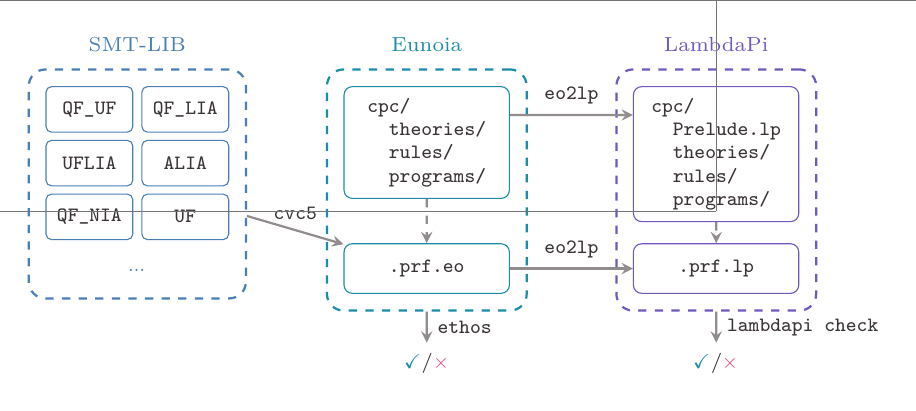
\begin{tikzpicture}[scale=1.05, every node/.style={transform shape},
		item/.style={draw, rounded corners=3pt, font=\scriptsize\ttfamily,
				align=left, inner sep=4pt, minimum height=0.6cm,
				minimum width=2.0cm, text=eoFgMath},
		frag/.style={draw, rounded corners=2pt, font=\scriptsize\ttfamily,
				inner sep=2pt, minimum height=0.55cm,
				minimum width=1.05cm, text=eoFgMath},
		arr/.style={->, thick, >=stealth, color=eoPunct},
		lbl/.style={font=\scriptsize, text=eoFgMath},
		box/.style={dashed, thick, rounded corners=6pt, inner sep=6pt}]
	% === Anchor grid: 3 columns, uniform spacing ===
	\def\colA{0}
	\def\colB{3.5}
	\def\colC{7}
	\def\lblY{1.55}
	% Label coordinates
	\coordinate (lblA) at (\colA,\lblY);
	\coordinate (lblB) at (\colB,\lblY);
	\coordinate (lblC) at (\colC,\lblY);
	% === Top-row alignment ===
	\def\topRowY{1.05}
	\def\botRowY{-0.85}
	% === SMT-LIB box (blue) ===
	% 3 rows evenly spaced using anchor=north, uniform gap
	\def\fragGap{0.65}
	\pgfmathsetmacro{\fragRowB}{\topRowY - \fragGap}
	\pgfmathsetmacro{\fragRowC}{\topRowY - 2*\fragGap}
	\node[frag, draw=eoAttr, anchor=north] (f1) at (\colA-0.58,\topRowY) {QF\_UF};
	\node[frag, draw=eoAttr, anchor=north] (f2) at (\colA+0.58,\topRowY) {QF\_LIA};
	\node[frag, draw=eoAttr, anchor=north] (f3) at (\colA-0.58,\fragRowB) {UFLIA};
	\node[frag, draw=eoAttr, anchor=north] (f4) at (\colA+0.58,\fragRowB) {ALIA};
	\node[frag, draw=eoAttr, anchor=north] (f5) at (\colA-0.58,\fragRowC) {QF\_NIA};
	\node[frag, draw=eoAttr, anchor=north] (f6) at (\colA+0.58,\fragRowC) {UF};
	% dots at center of where 4th row would be
	\pgfmathsetmacro{\fragRowD}{\topRowY - 3*\fragGap}
	\pgfmathsetmacro{\dotsY}{\fragRowD - 0.28}
	\node[lbl, text=eoAttr] (dots) at (\colA,\dotsY) {$\ldots$};
	\node[box, draw=eoAttr, fit=(f1)(f2)(f5)(f6)(dots)] (smtbox) {};
	\node[lbl, text=eoAttr] at (lblA) {SMT-LIB};
	% === EO box (teal) ===
	\node[item, draw=eoBuiltin, anchor=north] (cpc) at (\colB,\topRowY)
	{cpc/%
		\\~~theories/\\~~rules/\\~~programs/};
	\node[item, draw=eoBuiltin, anchor=north] (prf) at (\colB,\botRowY) {.prf.eo};
	\node[box, draw=eoBuiltin, fit=(cpc)(prf)] (eobox) {};
	\node[lbl, text=eoBuiltin] at (lblB) {Eunoia};
	% === SMT -> EO: cvc5 ===
	\draw[arr] (smtbox) -- node[above, font=\scriptsize\ttfamily, text=eoFgMath] {cvc5} (prf);
	% === cpc -> prf.eo (dependency) ===
	\draw[arr, dashed] (cpc) -- (prf);
	% === EO -> check (ethos) ===
	\node[lbl] (chk1) at (\colB,-2.3) {{\color{eoBuiltin}$\checkmark$}/{\color{eoKeyword}$\times$}};
	\draw[arr] (eobox) -- node[right, font=\scriptsize\ttfamily, text=eoFgMath] {ethos} (chk1);
	% === LP box (purple) ===
	\node[item, draw=eoConst, anchor=north] (cpclp) at (\colC,\topRowY)
	{cpc/%
		\\~~Prelude.lp\\~~theories/\\~~rules/\\~~programs/};
	\node[item, draw=eoConst, anchor=north] (prflp) at (\colC,\botRowY) {.prf.lp};
	\node[box, draw=eoConst, fit=(cpclp)(prflp)] (lpbox) {};
	\node[lbl, text=eoConst] at (lblC) {LambdaPi};
	% === cpc-lp -> prf.lp (dependency) ===
	\draw[arr, dashed] (cpclp) -- (prflp);
	% === EO -> LP: eo2lp ===
	\draw[arr] (cpc.east |- cpc.north east) ++(0,-0.35) coordinate (eo2lp-l)
	-- node[above, font=\scriptsize\ttfamily, text=eoFgMath] {eo2lp}
	(cpclp.west |- eo2lp-l);
	\draw[arr] (prf.east) -- node[above, font=\scriptsize\ttfamily, text=eoFgMath] {eo2lp} (prflp.west);
	% === LP -> check (lambdapi) ===
	\node[lbl] (chk2) at (\colC,-2.3) {{\color{eoBuiltin}$\checkmark$}/{\color{eoKeyword}$\times$}};
	\draw[arr] (lpbox) -- node[right, font=\scriptsize\ttfamily, text=eoFgMath] {lambdapi check} (chk2);
\end{tikzpicture}
}
\end{boxfigure}
% ---------------------------------------------------------

\subsubsection{Contribution.}
Our work has a dual role.
Practically, \texttt{eo2lp} (\autoref{sec:results})
provides an independent type-theoretic proof checker
for \cvc{5}, translating all 22~modules of CPC-MINI
(359~rules, 96~programs, 57~constants) and verifying
97\% of 1{,}036~proof scripts across 14~SMT-LIB fragments.
%
Conceptually, the translation gives a
\emph{typed interpretation} of Eunoia in the
$λΠ$-calculus, where Eunoia sorts become elements of a
Tarski universe~$\Set$ with carrier~$\msf{τ}$,
inference rules become axioms, and side-condition
programs become rewrite rules whose type preservation
is checked by LambdaPi.
%
This parallels SMT-LIB's model-theoretic semantics
where sorts are interpreted as sets, and is a step
towards a formal semantics for the still-evolving
Eunoia language.

The paper is organised as follows.
\Autoref{sec:eunoia} formalizes the fragment of
Eunoia used by \cvc{5}---its term syntax, command
structure, and elaboration semantics.
%
\Autoref{sec:lambdapi} defines the translation
of Eunoia into the $λΠ$-calculus modulo rewriting,
covering inference rules, side-condition programs,
and elaboration uniformly so that \cvc{5}'s entire
proof system is encoded automatically rather than
rule-by-rule.
%
\Autoref{sec:results} describes \texttt{eo2lp}
and reports the benchmark results.

\subsubsection{Related Work.}
Coltellacci et
al.~\cite{coltellacciReconstructionSMTProofs2024a,coltellacci25frocos}
reconstruct Alethe~\cite{schurrAletheGenericSMT2021}
proofs from
\cvc{5}~\cite{Barbosa2022}
in LambdaPi via hand-written soundness lemmas for each
Alethe rule, covering UF and linear integer arithmetic.
%
Similarly, \textsc{lean-smt}~\cite{mohamed25leansmt}
covers ${\sim}200$ of the 662~CPC rules
(${\sim}30\%$) by interactively proving each rule
sound in Lean~4, then automating the translation
of cvc5 proofs that use them.
%
Our work instead targets Eunoia as a framework:
all 359~CPC-MINI rules are translated automatically as
\emph{axioms} in LambdaPi, without per-rule soundness
proofs, but whose well-typedness and subject reduction
are verified.

The idea of reducing SMT proof checking to type
checking originates with
LFSC~\cite{DBLP:journals/fmsd/StumpORHT13};
Eunoia inherits this approach and extends it with
the higher-order features similar to those of
the speculative SMT-LIB~3
proposal~\cite{barrettSMTLIB3Bringing,smt3-proposal,barbosa17hosmt}.
%
Brown~\cite{Brown2021} argues that this expressive
type system calls for proof representations in
type-theoretic frameworks; our encoding realizes
this idea using the $λΠ$-calculus.
%
SMT proof reconstruction is also used within
proof assistants:
Isabelle/HOL replays Alethe
proofs~\cite{DBLP:conf/cade/SchurrFD21,lachnitt25isabelle},
SMTCoq~\cite{ekici17smtcoq} integrates solvers
into Rocq, and
IsaRare~\cite{lachnitt24isarare} verifies
CPC rewrite rules in Isabelle/HOL.

The Dedukti ecosystem serves as an
interoperability hub for proof assistants
(Rocq~\cite{boespflug12coqine},
Isabelle~\cite{isabelle_dedukti},
HOL~Light~\cite{assaf15translating},
Matita~\cite{krajono},
Lean~\cite{vaishnav25lean4less})
and automated provers
(iProverModulo~\cite{burel20first},
ArchSAT~\cite{bury:tel-02612985},
Vampire~\cite{komel2025case},
TPTP~\cite{DBLP:conf/flairs/SutcliffeBB25});
our work extends this ecosystem to SMT via
the Eunoia framework.

% ---------------------------------------------------------
% Placed here so it floats to the top of page 2
\begin{boxfigure}[t!]{fig:eo-syntax}
	{Syntax for Eunoia: terms, attributes, and built-in operators.}
	\alttext{Three stacked grammar tables for Eunoia.
		Top: term syntax---terms are symbols, literals, applications, or
		binder applications; parameters carry an optional attribute (:implicit, :list).
		Middle: constant attributes---right/left-associative (with optional nil terminator),
		chainable, pairwise, binder, arg-list.
		Bottom: built-in symbols grouped by family---core (eo::eq, eo::requires, eo::quote,
		eo::var), boolean (eo::and, eo::or, eo::not, eo::xor),
		arithmetic (eo::add, eo::mul, eo::neg, eo::zdiv), and
		list (eo::nil, eo::cons, eo::list\_concat, eo::list\_len).}{%
		\vspace{4pt}\centerline{$\eoTermSyntax$}
		\boxfigurehline
		\centerline{$\eoAttrSyntax$}
		\boxfigurehline
		\centerline{$\eoBuiltinFig$}\vspace{4pt}}
\end{boxfigure}
% ---------------------------------------------------------

\end{document}
